\documentclass[../main.tex]{subfiles}
\begin{document}
\subparagraph{Problem 2}\label{subpar:problem2_rom}

Contrary to problem $1.$ here the reduced dynamical system does have a time dependence since we included transient solutions in the snapshot matrix $\boldsymbol{X}$.
We thus assemble \eqref{eq:reduced_dynamical_system} and solve it forward in time using again the Euler implicit time stepping scheme introduced above for the evolution of the FOM

\begin{figure}[H]
    \centering 
    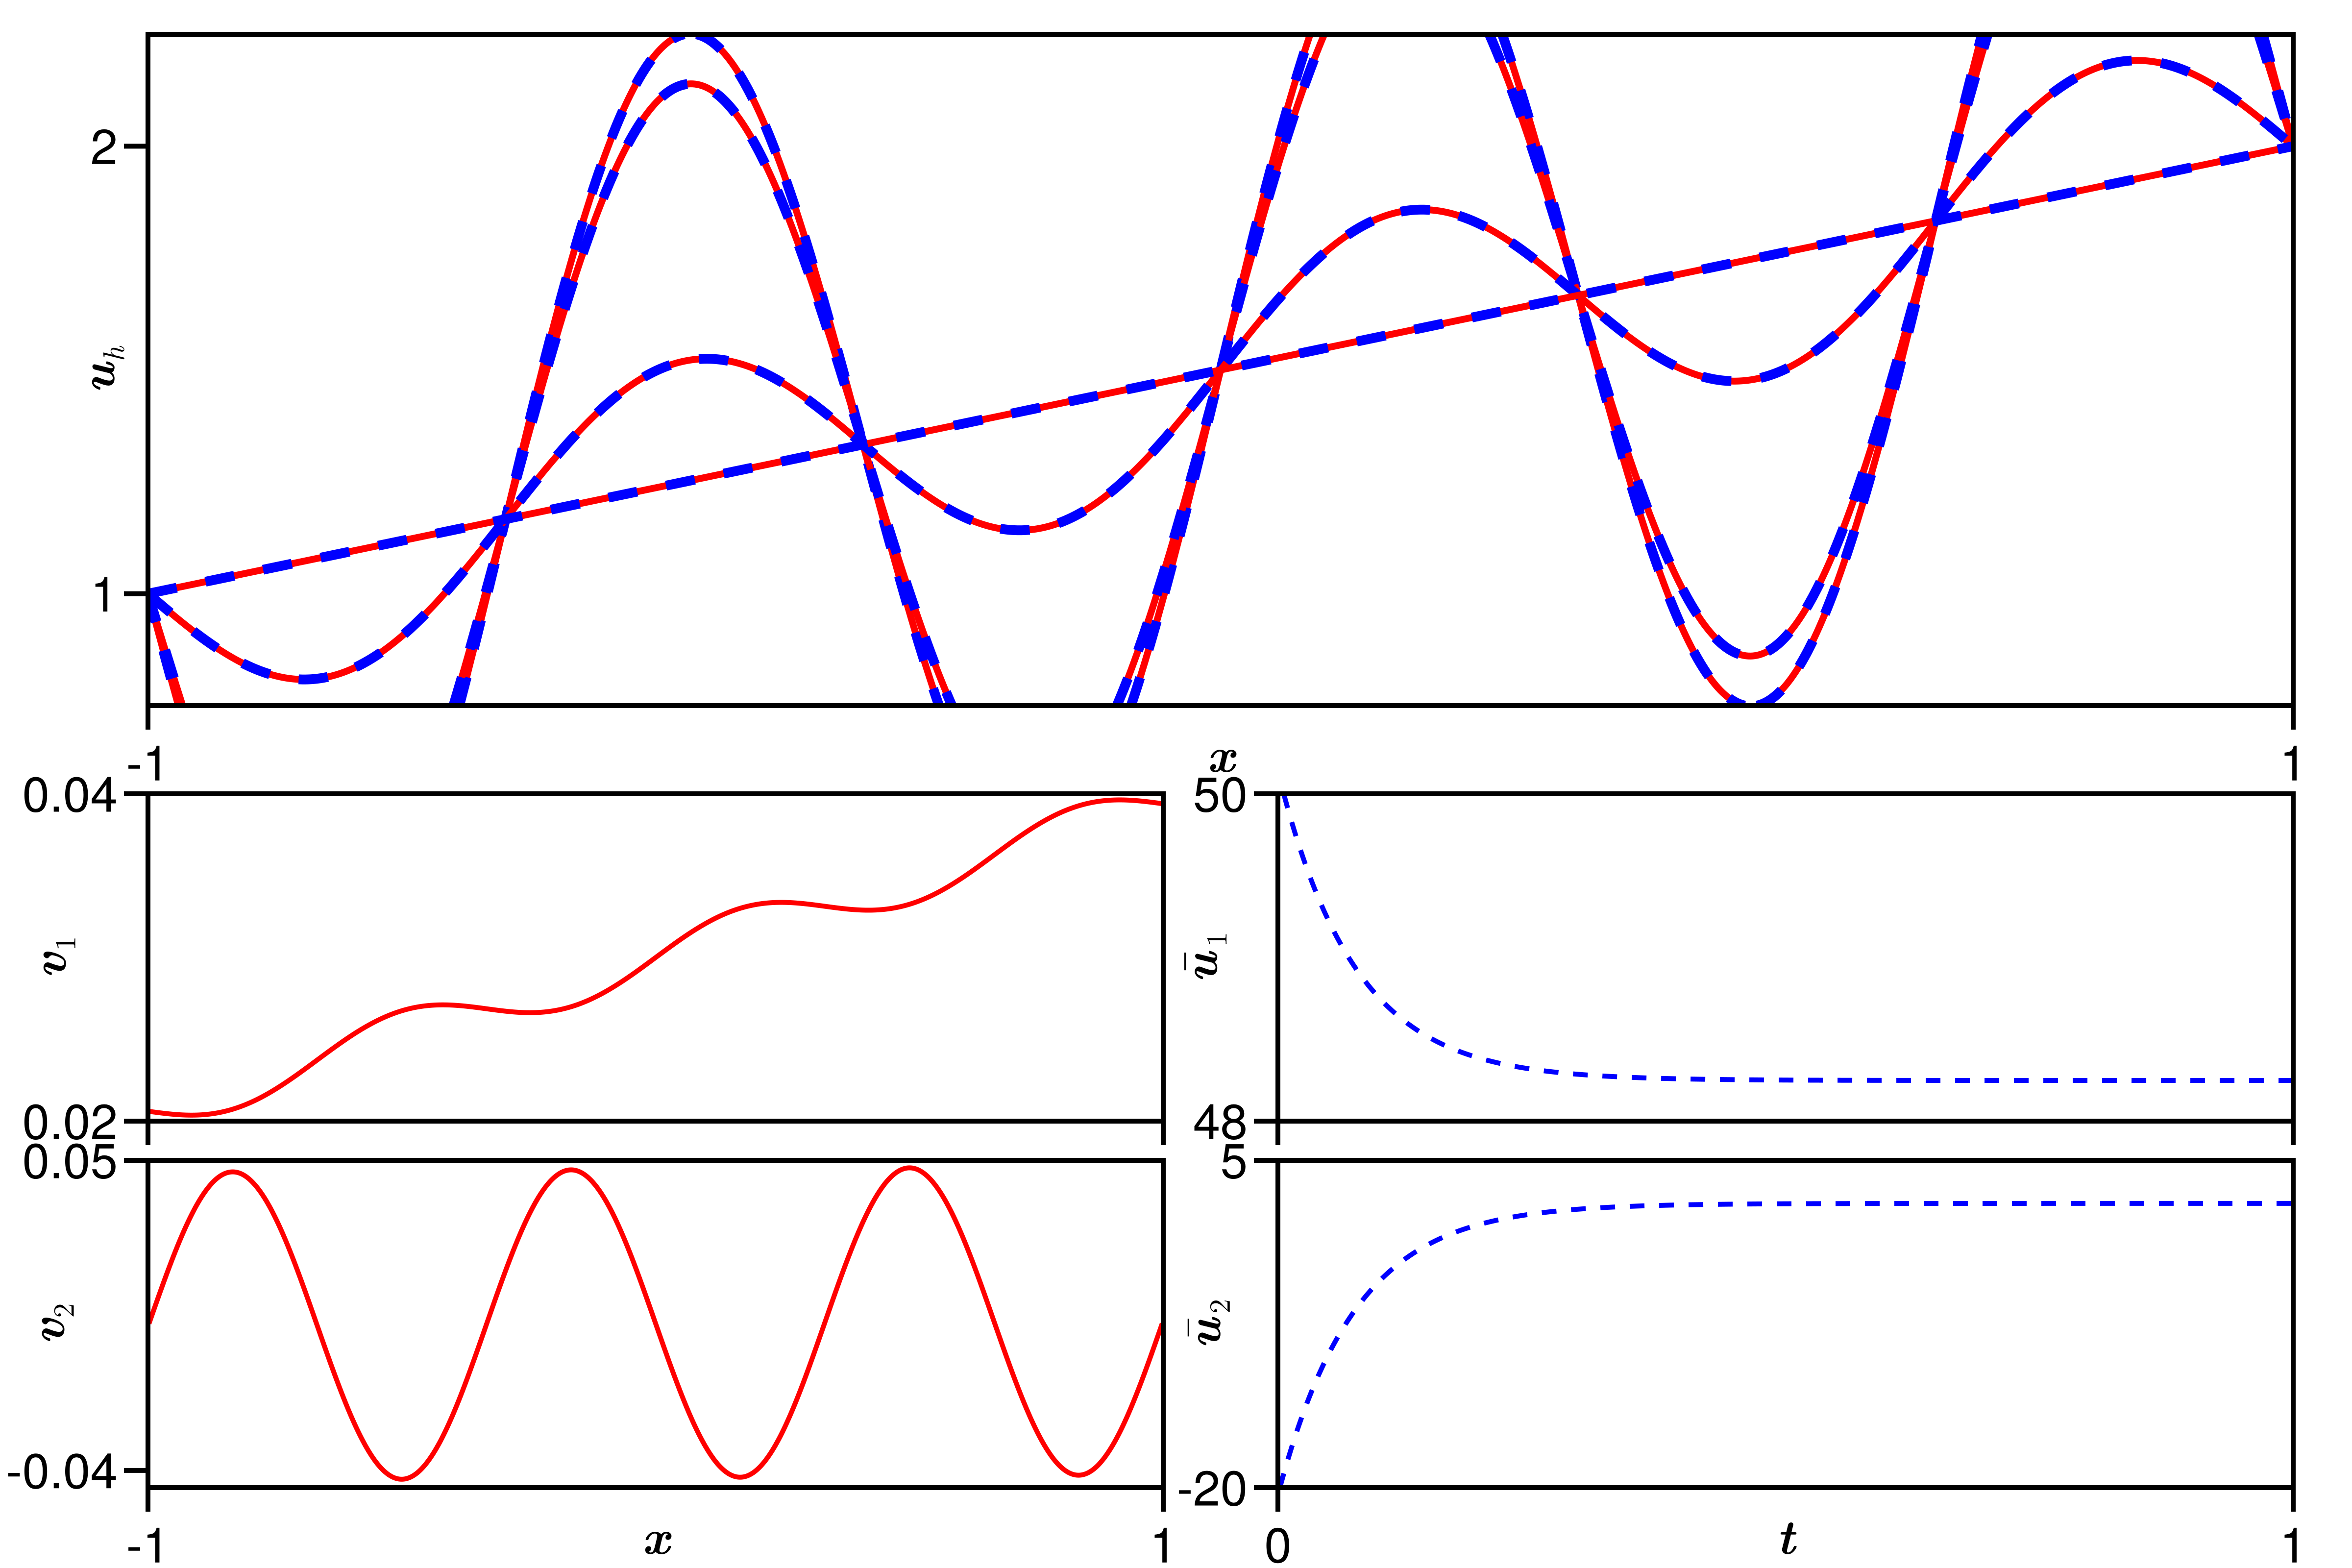
\includegraphics[keepaspectratio, width=0.75\textwidth]{../figures/fig:problem2_rom.png}
    \caption{\textbf{Top}: comparison between the FOM time-evolution (dashed, red) and the reduced-order (dashed, blue) approximation at parameter value $\mu=0.15$.
    \textbf{Bottom}: stationary singular vectors (left) forming the basis of $\mathcal{R}_{h}$ and time-dependent coefficients (right) of the affine expansion of the solution in such basis.}
    \label{fig:problem2_rom}
\end{figure}

In Figure \ref{fig:problem2_rom} we observe how the linear superposition of two basis vectors is capable of reproducing the same time evolution of the FOM.
The Kolmogoroff $n-$width decay is reported in Figure \ref{fig:problem2_decay} 

\begin{figure}[H]
    \centering 
    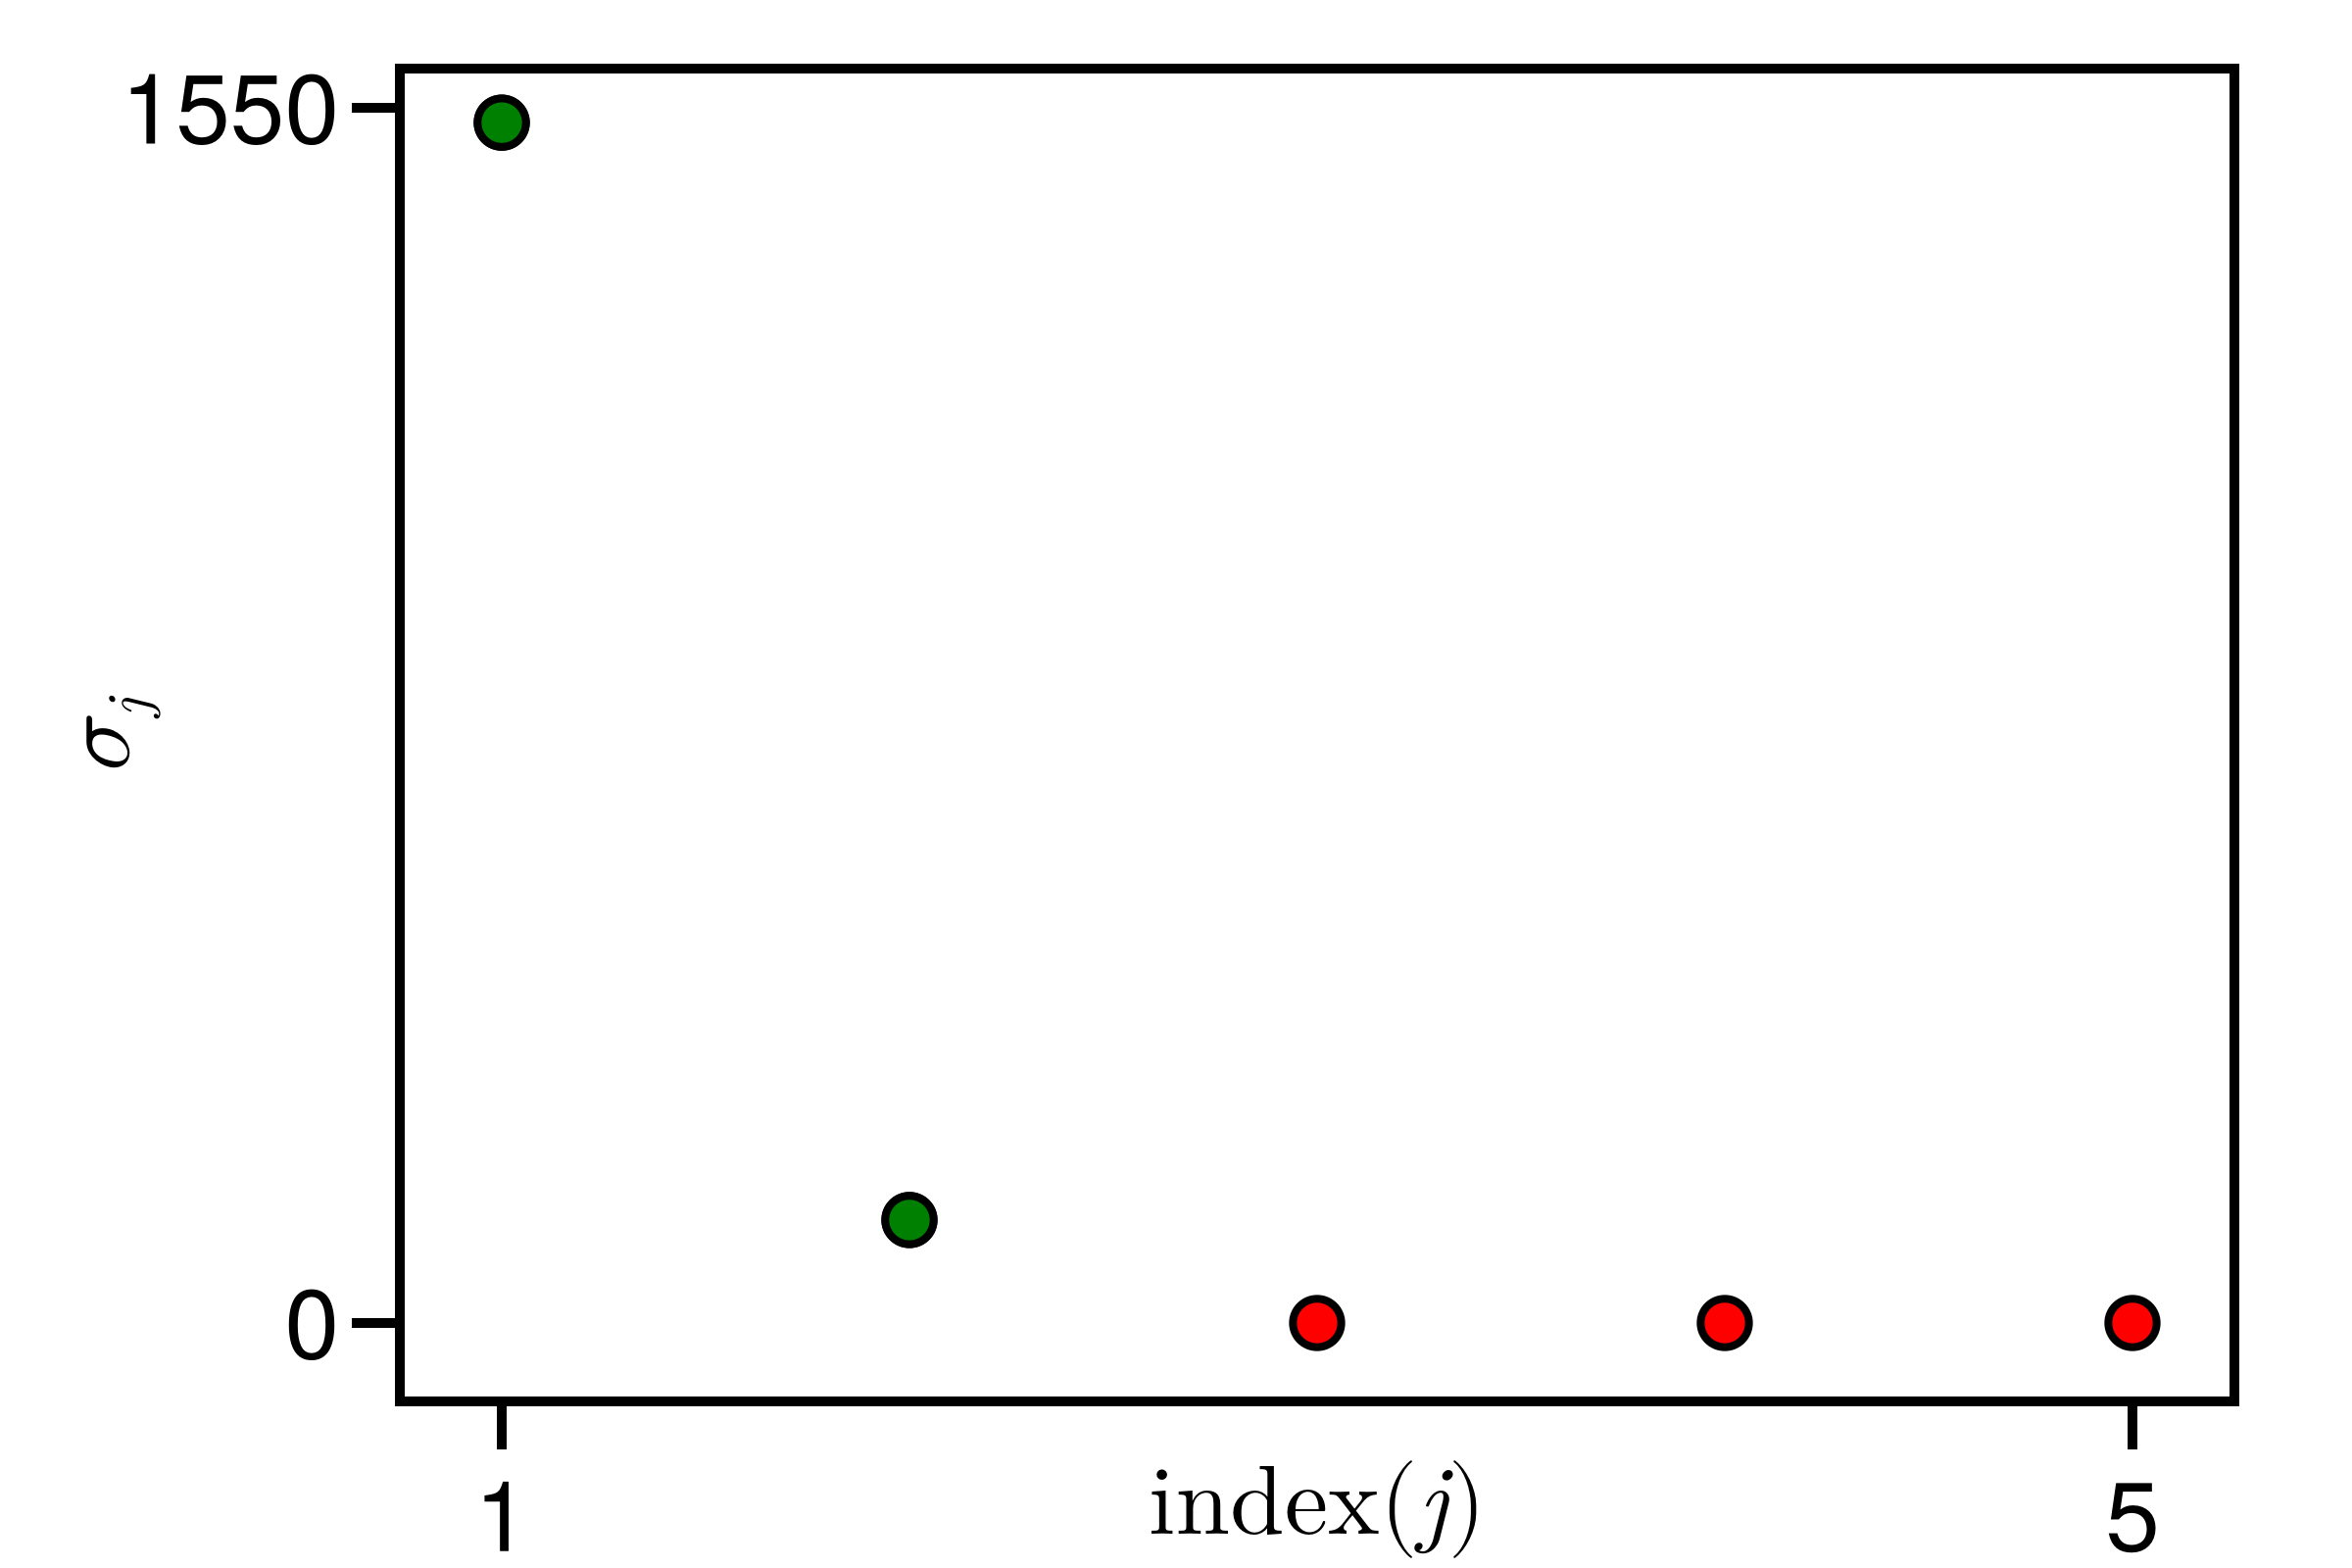
\includegraphics[keepaspectratio, width=0.7\textwidth]{../figures/fig:problem2_decay.png}
    \caption{Kolmogoroff $n-$width decay of problem $2.$ of \eqref{eq:heat}. Green dots reppresent the $N_{r}=2$ singular values used for constructing the ROM.}
    \label{fig:problem2_decay}
\end{figure}

\end{document}
